%experimental.tex
\section{Experimental Evaluation: \\3-\acs{DOF}  \acs{UV} Rotational Dynamics \acs{AID}}
\label{chUV_AID.sec.UVSO3exp}

This Section reports a comparative experimental evaluation of \ac{AID}
and \ac{LS} for the estimation of plant parameters for the rotational
dynamics of a \ac{UV}.
%
We employed the Johns Hopkins University Hydrodynamic Test Facility to
evaluate each parameter identification method's capacity to identify
parameter sets which accurately model \ac{UV} dynamics.
%
The error between the predicted model performance and the
experimentally observed performance is reported as the \ac{MAE}
between the simulated plant roll, pitch, and velocities and the actual
experimental plant roll, pitch, and velocities.
%
Appendices \ref{appenJHUHTF.sec.hydrolab}
and \ref{appenJHUHTF.sec.paramEvalMethod} provide further details about
our experimental setup and parameter evaluation method.


At the beginning of each experiment, the vehicle was positioned in the
center of the tank with the vehicle's depth under closed loop control
at about a \unit{1}{\m} depth with the x and y \ac{DOF} unactuated.
%
During the experiment three sinusoidal torque commands (one in the
direction of each axis of the vehicle's coordinate frame) actuated the
angular position of the \ac{JHUROV}.
%
Table \ref{chUV_AID.tb.UVSE3expStat} shows the details of two exogenous
inputs, one for system identification and one for cross validation.
%
Hereafter we will refer to these experiments as the \ac{IDDAT} and the
\ac{CROSS} respectively.



\begin{table}[htbp]
\ssp
\caption{Exogenous Inputs for \ac{UV} Rotational Dynamics Parameter
  Identification Experiments}  
\begin{center}
\begin{tabular}{cccc}
\multicolumn{2}{c}{Experiment} & \ac{IDDAT} & \ac{CROSS} \\
\hline
\multicolumn{2}{c}{Experiment Purpose}  & Parameter      & Parameter  \\
               &                        & Identification & Cross-Validation \\
\hline
\multicolumn{2}{c}{Experiment Date}     & 2012-04-14    &   2012-04-09  \\ 
\hline
\multicolumn{2}{c}{Experiment Run Time} &  22.0 min     &   21.7 min    \\ 
\hline
Torque about &          Cos Freq          & 0.503 rad/sec & 0.583 rad/sec \\ 
X Vector     &          Cos Amp           &     40 N m    &     40 N m    \\ 
\hline
Torque about &          Cos Freq          & 0.663 rad/sec & 1.012 rad/sec \\ 
Y Vector     &          Cos Amp           &     55 N m    &     55 N m    \\ 
\hline
Torque about &          Cos Freq          & 1.043 rad/sec & 0.733 rad/sec \\ 
Z Vector     &          Cos Amp           &     70 N m    &     70 N m    \\ 
\hline \end{tabular}
\end{center}
\label{chUV_AID.tb.UVSO3expStat}
\end{table}



\begin{table*}[htbp]
\ssp
\caption{Numerical Values of the \ac{INITP} used to initialize \ac{UV} rotational dynamics \ac{AID}.}
\begin{center}
\begin{tabular}{c|c}
Parameter Symbol & \acf{INITP} \\ \hline
$\hat{I}(t_0)$ &
$ \left[\begin{array}{ccc} 100.0 & 0 & 0\\ 0 & 100.0 & 0\\ 0 & 0 & 100.0 \end{array}\right] $
\\
$\hat{C}_1(t_0)$ &
$ \left[\begin{array}{ccc} -100.0 & 0 & 0\\ 0 & -100.0 & 0\\ 0 & 0 & -100.0 \end{array}\right] $
\\
$\hat{C}_2(t_0)$ &
$ \left[\begin{array}{ccc} -100.0 & 0 & 0\\ 0 & -100.0 & 0\\ 0 & 0 & -100.0 \end{array}\right] $
\\
$\hat{C}_3(t_0)$ &
$ \left[\begin{array}{ccc} -100.0 & 0 & 0\\ 0 & -100.0 & 0\\ 0 & 0 & -100.0 \end{array}\right] $
\\
$\hat{b}(t_0)$ &
$ \left[\begin{array}{c} 0\\ 0\\ 100.0 \end{array}\right] $
\\
\end{tabular}
\end{center}
\label{chUV_AID.tb.UVSO3_INIT_params}
\end{table*}



\ac{AID} was implemented as a discrete time approximation of the
continuous time algorithm.  
%
%Once every 100ms the most recent state measurements, commanded torque,
%parameter estimates, and angular velocity estimate were used to
%calculate the angular velocity and parameter estimate derivatives
%(\ref{chUV_AID.eq.UV_SO3_Estimator})-(\ref{chUV_AID.eq.UV_SO3_BuoyId}).
%
Euler integration of (\ref{chUV_AID.eq.UV_SO3_Estimator})---(\ref{chUV_AID.eq.UV_SO3_BuoyId})
for 100ms time steps
provided the time series of parameter and angular velocity
estimates.
%
100ms is one to two orders-of-magnitude smaller than the state signal
variation rates of 1 second or greater observed during quasi-periodic
\ac{JHUROV} operations.
%
The experiments were designed to generate thruster commands varying
slowly enough to admit the use of steady state thruster models.
%
In practice, first-order Euler integration provided performance
similar to the 4th-order integration implemented in simulation.



The \ac{AID} algorithm was initialized with the measured angular position,
measured angular velocity, and \acf{INITP} in Table
\ref{chUV_AID.tb.UVSO3_INIT_params}.
%
Note that the \ac{INITP} was chosen such that each scalar
parameter was within an order-of-magnitude of the value to be identified.
%
The choice of optimal adaptation gains is a long-standing open problem
in adaptive systems theory\cite{Nguyen-2009,ksn&anu.book}.
%
From simulations of this \ac{AID} algorithm which sparsely covered a 
roughly logarithmic scaling for a range of possible gains, we
empirically chose angular velocity, inertia tensor, quadratic drag,
and buoyancy torque adaption gains of $a=10$, $\gamma_1=5000$,
$\gamma_2=10000$, and $\gamma_3=1000$ respectively.
%
Many of the gain combinations considered provided parameter
convergence rates comparable to the gains used herein.
%
Our simulation studies suggest similar results would be obtained for
initial condition and gain choices within an order-of-magnitude of the
choices made.





\subsection{Experimental Results}%\label{ref.expResults}


The state measurements from the \ac{IDDAT} dataset were used to
identify the plant parameters of the plant model
(\ref{chModels.eq.UVSO3plant}) with both the adaptive identification
and least squares methods.
%
Table \ref{chUV_SO3.tb.UVSO3_ID_params} reports two identified
parameter sets: the \acf{AIDP} estimated with \ac{AID} (as per Section
\ref{chUV_AID.sec.UV_SO3_AID}) and the \acf{LSP} estimated with
\ac{LS} (as per Section \ref{chUV_AID.sec.leastSquares}). 
%TM_CHECK could cut out the 'as per' parenthetal statements above 
%

The parameter sets \ac{AIDP},  \ac{LSP}, and \ac{INITP} were used as
parameter sets for three \ac{UV} rotational dynamics models; the
\acf{AIDPM}, the \acf{LSPM}, and the \acf{INITPM}.
%
Using the torque input commands from the \ac{IDDAT} and \ac{CROSS}
datasets, we compare simulated \ac{JHUROV} performance from numerical
simulations of \ac{AIDPM}, \ac{LSPM}, and \ac{INITPM} to the measured
\ac{JHUROV} states for each experiment respectively.

Using the torque inputs from the \ac{CROSS} dataset, Figures
\ref{chUV_AID.fig.SO3_INIT_pos} --- \ref{chUV_AID.fig.SO3_AID_vel}
compare the state measurements from simulations of \ac{AIDPM},
\ac{LSPM}, and \ac{INITPM} to the measured \ac{JHUROV} states from
the \ac{CROSS} dataset.
%
%The \ac{JHUROV} simulation in Figures \ref{chUV_AID.fig.SO3_INIT_pos}
%and \ref{chUV_AID.fig.SO3_INIT_vel} use the \ac{INITP} to model
%vehicle dynamics.  
%
%In a similar fashion, Figures \ref{chUV_AID.fig.SO3_AID_pos} and
%\ref{chUV_AID.fig.SO3_INIT_vel} plot data from two \ac{JHUROV}
%simulations, using either the \ac{AIDP} or \ac{LSP} to model vehicle
%dynamics.
%
Each of these four Figures display three minute subsets of the 20 minutes of
state data generated by driving simulations of \ac{AIDPM},
\ac{LSPM}, and \ac{INITPM} using the torque data from the \ac{CROSS}
dataset.
%
Similar simulations of \ac{AIDPM}, \ac{LSPM}, and \ac{INITPM} were
created using the torque commands from the \ac{IDDAT} dataset.
%
Table \ref{chUV_AID.tb.SO3_MAE} summarizes the \ac{MAE} between
measured and simulated vehicle state for each experimental dataset,
%(\ac{IDDAT} or \ac{CROSS)), 
\ac{UV} vehicle model, 
%(\acf{AIDPM}, \acf{LSPM}, and \ac{INITPM}), 
and open-loop-stable \ac{DOF}.
%(roll, pitch and agular velocities).


\begin{table}[htbp]
\ssp
\caption{\acfp{MAE} between measured and simulated vehicle states for all pairs of 
  \ac{UV} rotational dynamics experiments and \ac{UV} rotational dynamics models.}
\begin{center}
\begin{tabular}{c|cccccc}
\ac{UV} & & \multicolumn{2}{c}{Angular Pose} & \multicolumn{3}{c}{Angular Velocity} \\ 
 Model & Experiment & Roll & Pitch & x \ac{DOF} & y \ac{DOF} & z \ac{DOF} \\ \hline
\ac{AIDPM}  & \ac{CROSS} & 4.11$^\circ$ & 2.88$^\circ$ & 6.16$^\circ$/s & 2.83$^\circ$/s & 3.44$^\circ$/s \\
\ac{LSPM}   & \ac{CROSS} & 2.50$^\circ$ & 2.65$^\circ$ & 3.36$^\circ$/s & 3.69$^\circ$/s & 5.46$^\circ$/s \\
\ac{INITPM} & \ac{CROSS} & 13.3$^\circ$ & 14.6$^\circ$ & 8.86$^\circ$/s & 12.9$^\circ$/s & 7.00$^\circ$/s \\
\ac{AIDPM}  & \ac{IDDAT} & 3.44$^\circ$ & 2.06$^\circ$ & 4.80$^\circ$/s & 1.99$^\circ$/s & 4.03$^\circ$/s \\
\ac{LSPM}   & \ac{IDDAT} & 2.08$^\circ$ & 1.76$^\circ$ & 2.45$^\circ$/s & 2.19$^\circ$/s & 5.05$^\circ$/s \\
\ac{INITPM} & \ac{IDDAT} & 14.8$^\circ$ & 17.1$^\circ$ & 8.83$^\circ$/s & 10.7$^\circ$/s & 6.32$^\circ$/s \\
\end{tabular}
\end{center}
\label{chUV_AID.tb.SO3_MAE}
\end{table}

\begin{table*}[htbp]
\ssp
\caption{The \ac{UV} rotational dynamics parameter sets identified
  using the \ac{IDDAT} dataset.}
\begin{center}
\begin{tabular}{c|cc}
Parameter Symbol & \ac{AIDP} & \ac{LSP} \\ \hline
$\hat{I}(t_f)$ &
$ \left[\begin{array}{ccc} 136.0 & -12.7 & 2.89\\ -12.7 & 175.0 & -1.06\\ 2.89 & -1.06 & 160.0 \end{array}\right] $
&
$ \left[\begin{array}{ccc} 31.9 & -5.04 & 1.53\\ -5.04 & 55.9 & -6.19\\ 1.53 & -6.19 & 96.3 \end{array}\right] $
\\
$\hat{C}_1(t_f)$ &
$ \left[\begin{array}{ccc} -215.0 & 19.1 & 21.3\\ -23.0 & -243.0 & -10.1\\ 7.16 & -80.9 & -129.0 \end{array}\right] $
&
$ \left[\begin{array}{ccc} -297.0 & 4.14 & 1.32\\ 7.6 & -414.0 & -28.1\\ 150.0 & -165.0 & 52.3 \end{array}\right] $
\\
$\hat{C}_2(t_f)$ &
$ \left[\begin{array}{ccc} -137.0 & 39.8 & 46.5\\ -14.0 & -367.0 & -39.2\\ 15.0 & -117.0 & -186.0 \end{array}\right] $
&
$ \left[\begin{array}{ccc} -358.0 & 13.7 & 13.0\\ 91.8 & -266.0 & -20.5\\ 107.0 & -181.0 & -80.2 \end{array}\right] $
\\
$\hat{C}_3(t_f)$ &
$ \left[\begin{array}{ccc} -80.6 & 38.4 & -17.3\\ -2.0 & -287.0 & 19.6\\ 37.0 & -52.1 & -214.0 \end{array}\right] $
&
$ \left[\begin{array}{ccc} 3.4 & 18.9 & -9.58\\ -9.27 & -262.0 & 18.2\\ -70.0 & 34.8 & -252.0 \end{array}\right] $
\\
$\hat{b}(t_f)$ &
$ \left[\begin{array}{c} 1.57\\ -1.5\\ 277.0 \end{array}\right] $
&
$ \left[\begin{array}{c} 1.38\\ 1.11\\ 235.0 \end{array}\right] $
\\
\end{tabular}
\end{center}
\label{chUV_SO3.tb.UVSO3_ID_params}
\end{table*}


\begin{center}
\begin{figure}[htbp]
  \begin{center}
    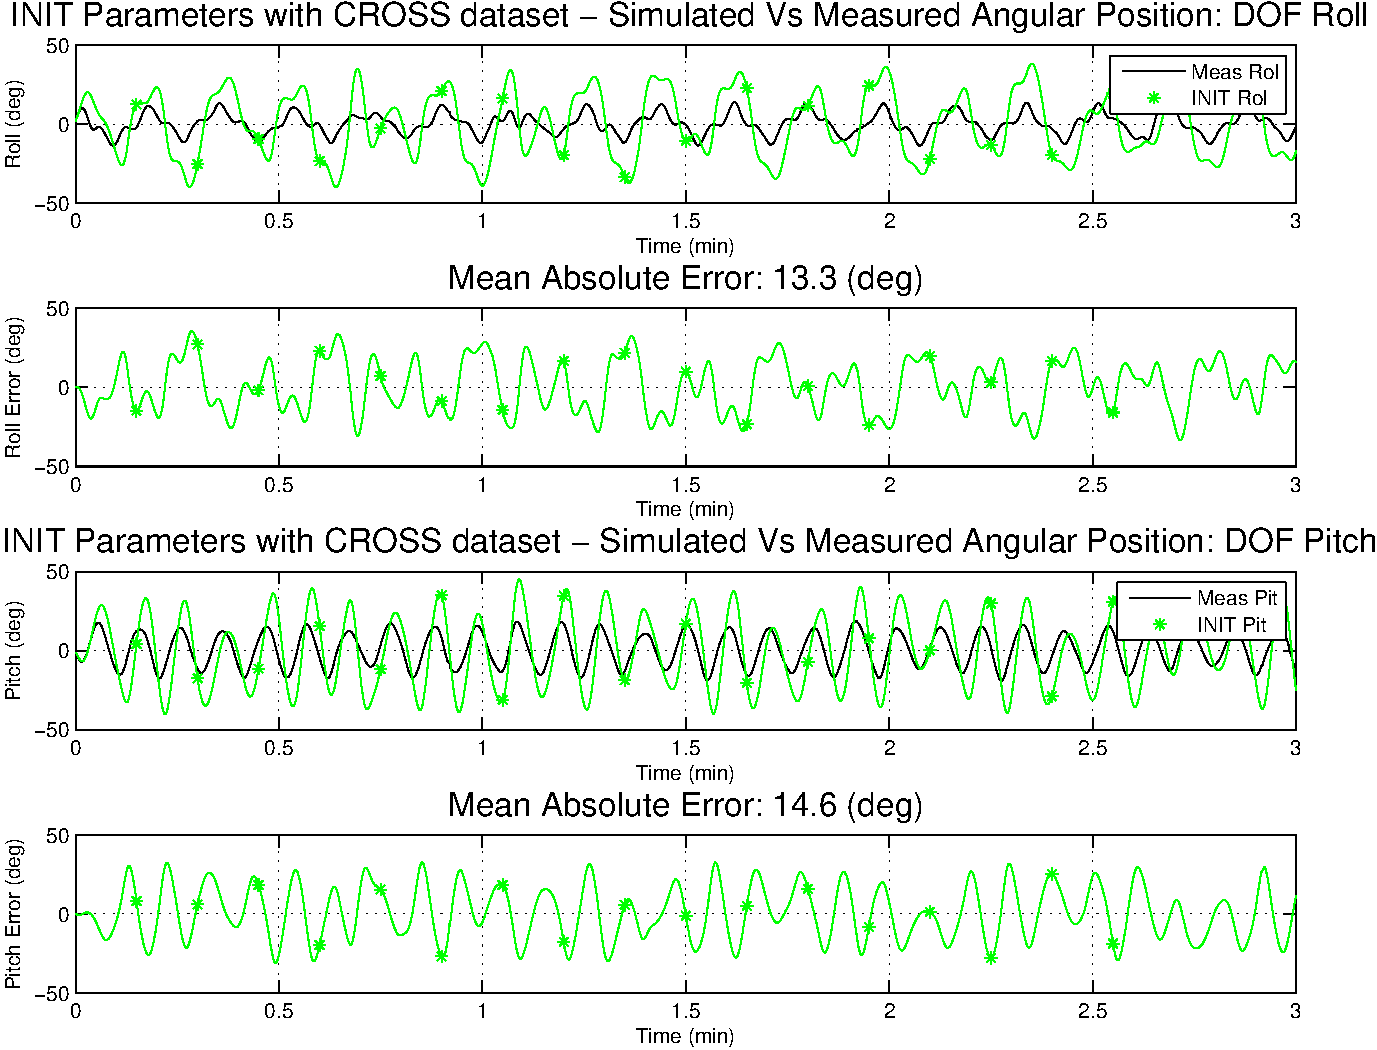
\includegraphics[width=6in]{./chUV_AID/images/crossINIT_pos}
  \end{center}
  \caption{ Representative data of experimental and simulated
    \ac{JHUROV} angular position for the \ac{CROSS} dataset. In the
    roll and pitch plots, the measured states are plotted together
    with the states from simulating \ac{INITPM}.  For each \ac{DOF},
    the difference between the measured position and simulated
    position is shown. 
%The \ac{INITP} was chosen to arbitrary
%    initialize the \ac{AID} algorithm, thus the large errors between
%    the simulated and measured angular positions of the \ac{JHUROV}
%    demonstrate there exists parameter sets which poorly characterize
%    the \acp{UV} performance.
}
  \label{chUV_AID.fig.SO3_INIT_pos}
\end{figure}
\end{center}

\begin{center}
\begin{figure}[htbp]
  \begin{center}
    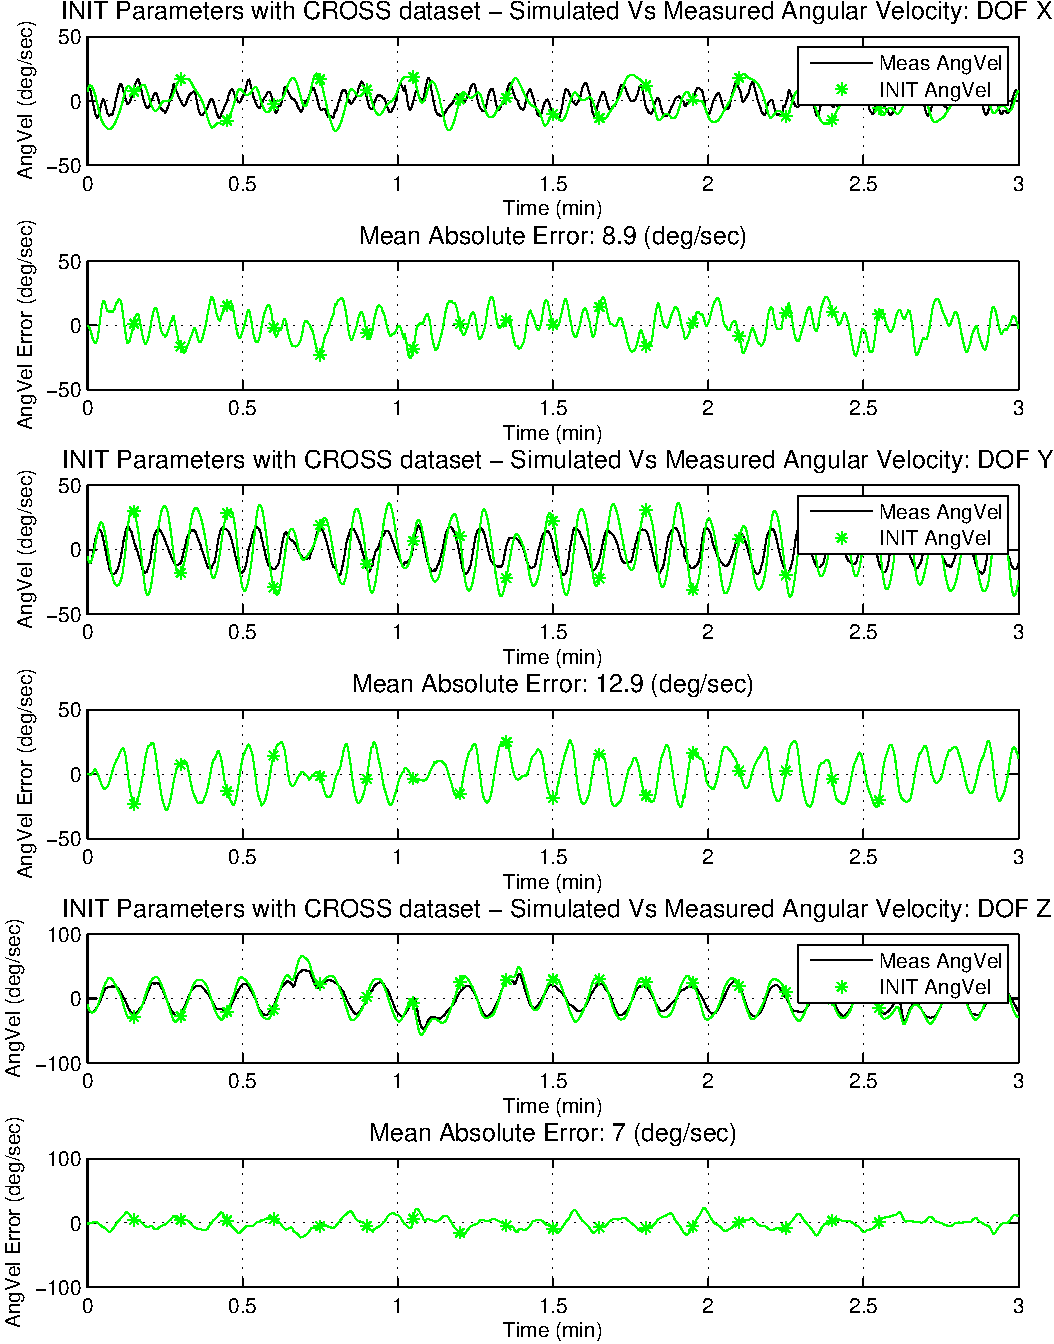
\includegraphics[width=5.5in]{./chUV_AID/images/crossINIT_vel}
  \end{center}
  \caption{ Representative data of experimental and simulated
    \ac{JHUROV} angular velocity for the \ac{CROSS} dataset. In the
    individual angular velocity plots, each measured velocity is
    plotted together with the states from simulating \ac{INITPM}.  For
    each \ac{DOF} error plots are also included. 
    %See the caption of
%    Figure \ref{chUV_AID.fig.SO3_INIT_pos} for further information.
}
  \label{chUV_AID.fig.SO3_INIT_vel}
\end{figure}
\end{center}

\begin{center}
\begin{figure}[htbp]
  \begin{center}
    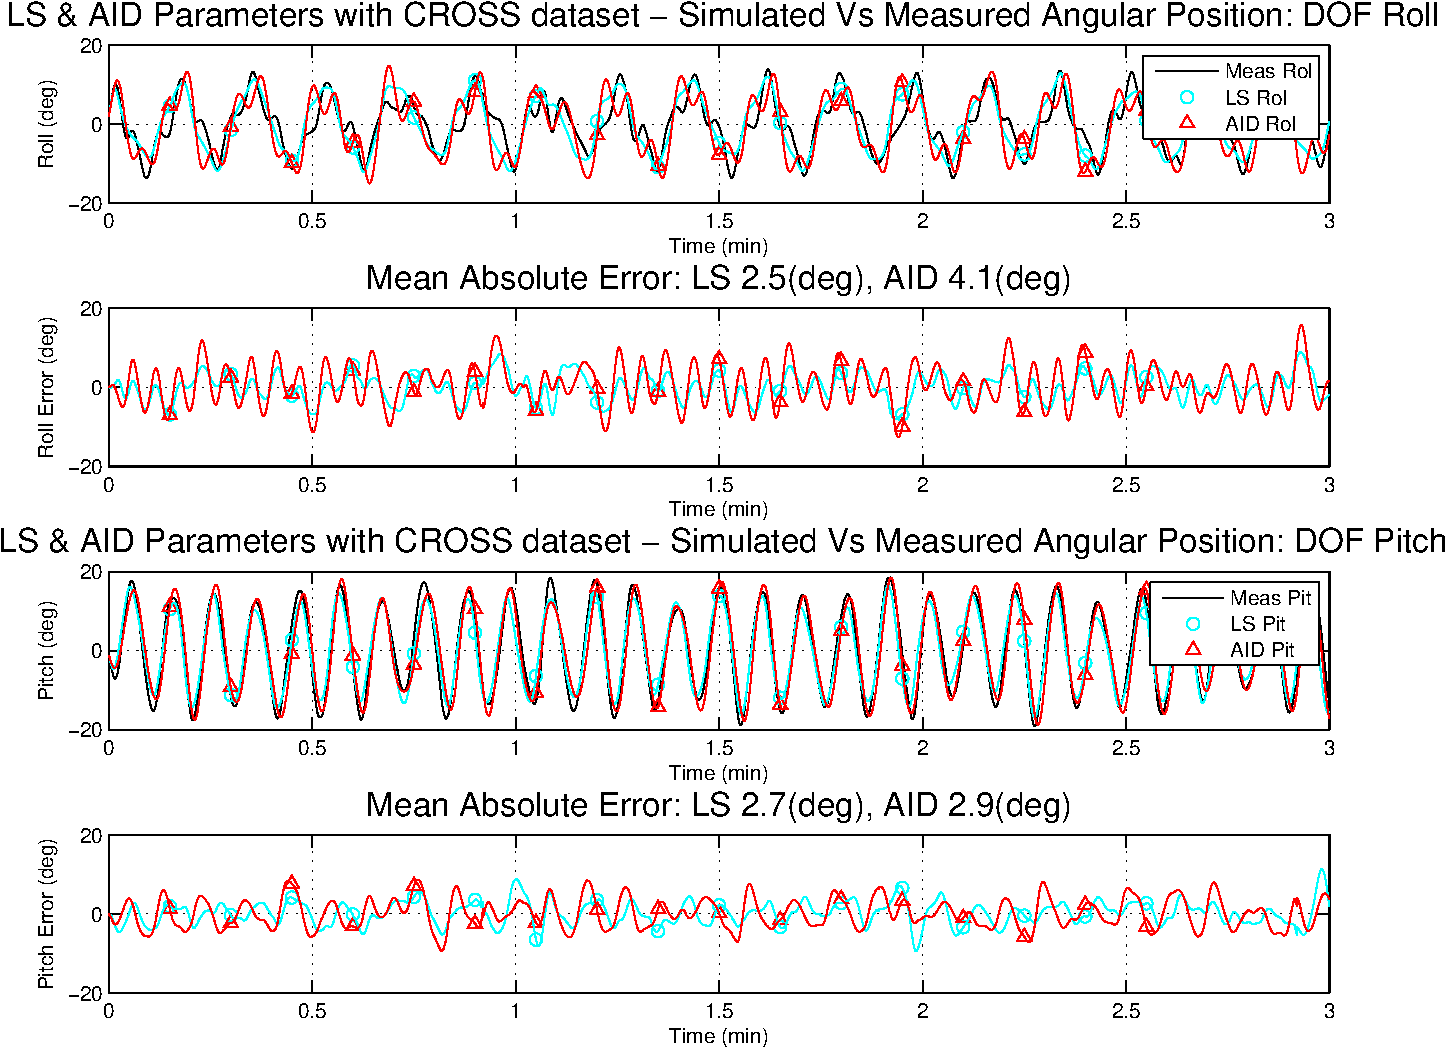
\includegraphics[width=6in]{./chUV_AID/images/crossAID_pos}
  \end{center}
  \caption{Representative data of experimental and simulated
    \ac{JHUROV} angular position for the \ac{CROSS} dataset. In the
    roll and pitch plots, the measured position is plotted together
    with the simulated position from two model simulations. The states
    from a simulation of \ac{AIDPM} are plotted in blue and marked with
    circles. The states from \ac{LSPM} are plotted in red and marked with
    triangles. For each \ac{DOF}, the difference between the measured
    positions from the \ac{CROSS} dataset and the states from each
    model simulation is shown.  For each \ac{DOF},
    the difference between the measured position and simulated
    position is shown. 
%Both models of the
%    \ac{JHUROV} provide a similar capacity to model the system, and
%    both perform better than the simulation using the arbitrary chosen
%    \ac{INITP} shown in Figures \ref{chUV_AID.fig.SO3_INIT_pos} and
%    \ref{chUV_AID.fig.SO3_INIT_vel}.  
}
  \label{chUV_AID.fig.SO3_AID_pos}
\end{figure}
\end{center}

\begin{center}
\begin{figure}[htbp]
  \begin{center}
    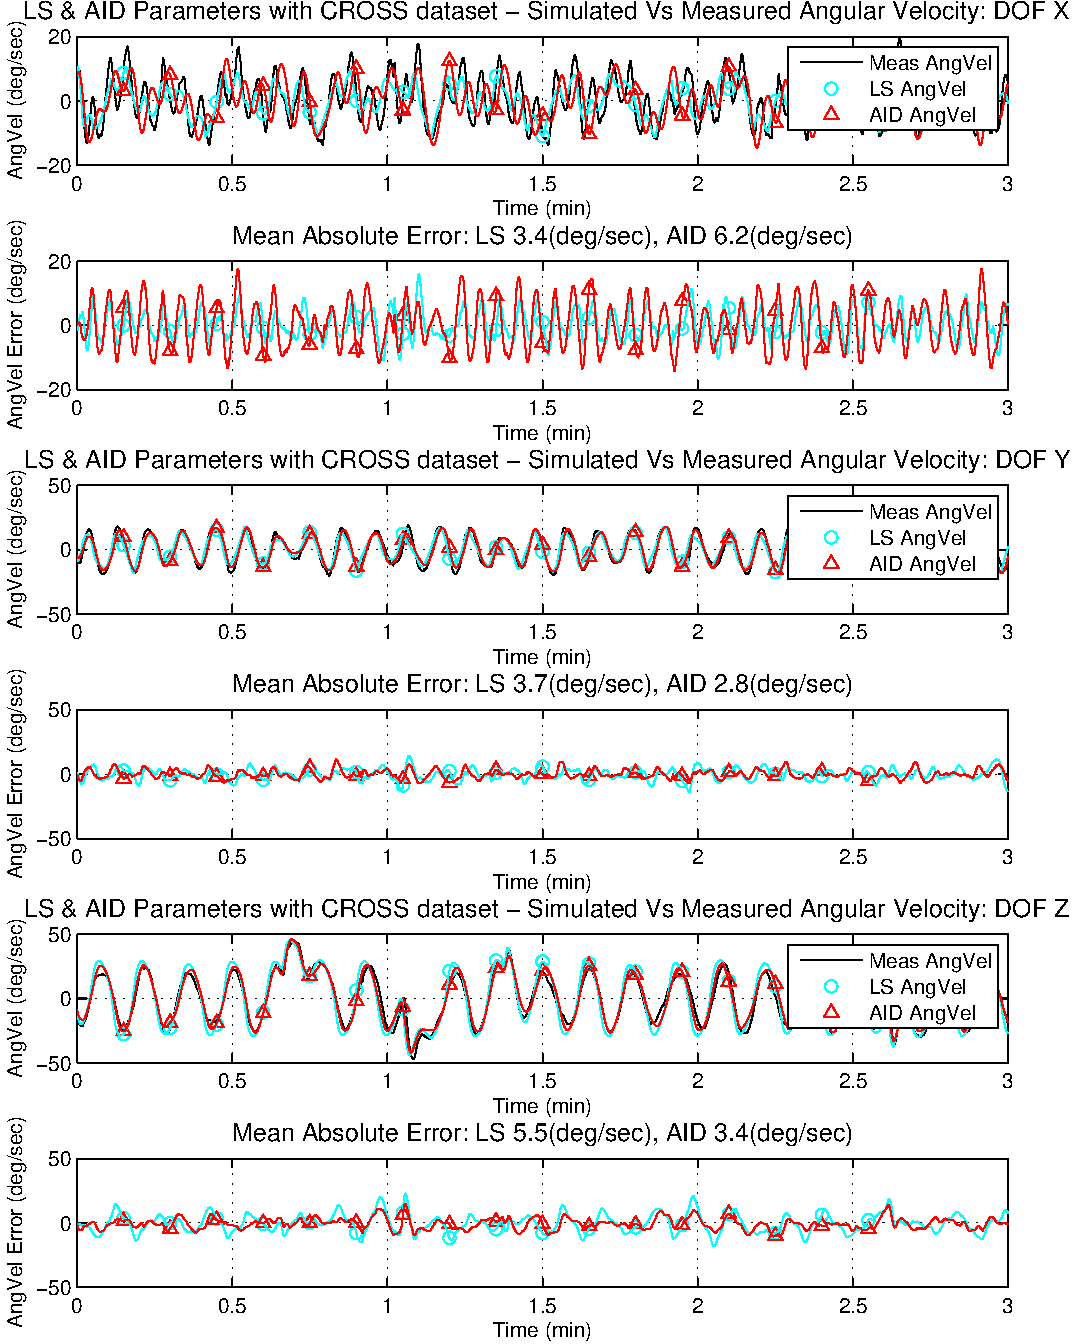
\includegraphics[width=5.5in]{./chUV_AID/images/crossAID_vel}
  \end{center}
  \caption{ Representative data of experimental and simulated \ac{JHUROV}
    angular velocity for the \ac{CROSS} dataset. In the
    individual angular velocity plots, each measured velocity is
    plotted together with velocities from \ac{AIDPM} and \ac{LSPM}
    simulations.  For each \ac{DOF} error plots are also included. See the
    caption of Figure \ref{chUV_AID.fig.SO3_AID_pos} for further information.}
  \label{chUV_AID.fig.SO3_AID_vel}
\end{figure}
\end{center}


% %TM_ENTIRE_UNCOMMENTED_PARAGRAPH_BELOW_ADDED_OK_WITH_LLW?
% Since there is only an emperical basis for using the analytic
% structure (\ref{eq.plantROV}) to model the dynamics of a
% \ac{UV}\cite{martin.thesis}, we are primarily conserned with finding plant
% parameters which match \ac{UV} dynamics over the range of possible
% torque inputs, as there could be a wide range of parameter sets which
% do so.
% %
% Therefore, we focus our analysis on the cross-validation experiment
% which was {\it not} used to identify parameter sets.
% %
% To judge the capacity of a parameter set to model the vehicle, we
% compare states estimated using a parameter set to the states recorded
% during a \ac{JHUROV} experimental run.
% %
% A good model, when used as an open loop observer, will provide
% accurate estimates of the pitch, roll and angular velocities of the
% vehicle when the vehicle's initial state and input torque history are
% used.
% %TM_COULD_ADD_THE_SENTENCE Because of the presence of a buoyancy
% %torque and the large effect of drag on \ac{UV} vehicle operation, the open
% %loop observer estimates can stay near the experimentially recorded
% %states even in the presence of moderate unmodeled exogenious torques. 
% %
% To create the open loop observer estimates \ac{UV} plant models
% (\ref{eq.plantROV}), one for each parameter set, were simulated using a 
% fourth order Runge Kutta numerical differential equation solver.  
% %
% The initial state provided to each simulation was that of the \ac{JHUROV}
% recorded at the start of the experiment, and the input torques used
% where those recorded by the \ac{JHUROV} control system during the
% duration of each experiment.
% %
% We report the mean absolute error (MAE) between each parameter set's
% simulated plant model and the corresponding expermentially observed
% plant states in Table \ref{chUV_AID.tb.SO3_MAE}.

%------------------------OLD_WORDS----------------------------------
% For comparative purposes we consider the differences between the
% values of states measured for \ac{JHUROV} and numerical simulations of
% the \ac{UV} plant model (\ref{eq.plantROV}) using one of the
% parameter sets in Table \ref{tb.paramSets}.
% %
% To simulate the \ac{JHUROV}'s trajectory for a given parameter set, a
% fourth order Runge Kutta numerical differential equation solver was
% used.
% % NEW WORDS
% Both the vehicle and the vehicle model have energy dissipation, an
% attractive equibium point in pitch and an attractive equibium point in
% roll. 
% %
% Because of these system traits, the effects of all previous
% events on the current roll, pitch, and angular velocities will lessen
% the further back in time an event occured. 
% %
% The more damping in a \ac{DOF}, the higher the energy dissipation, and the
% quicker previous events are forgotten.
% %
% If a perfect \ac{JHUROV} model and the \ac{JHUROV} itself are
% provided the same external torque signal, the states of both will
% match for all time.  
% %
% Differences in state which arise could be caused
% by several factors including noise (unmodeled external torques),
% mismatched parameter selection, or flawed model structure
% (\ref{eq.plantROV}).  
% %
% A single event for any of these factors could
% cause a nonzero error state.  
% %
% But since both the expermental and simulated \ac{JHUROV} are being driven
% by the same external torque, the interval of time over which a
% particular event can cause the roll, pitch, or angular velocity errors
% is finite.
% %
% Since modeling errors should be regularly causing differences in
% errors in state,  judging the typical error between the experimental
% and simulated \ac{JHUROV} states should allow us to characterize relative
% performance of each model.
% %
% Thus for pitch, roll, and each angular velocity \ac{DOF} we present plots
% of state, plots of error, and values of mean absolute error (MAE) to
% characterize the relative performance of each model.



\subsection{Analysis of Experimental Results}

Compare the state estimate capacity of \ac{INITPM} in Figures
\ref{chUV_AID.fig.SO3_INIT_pos} and \ref{chUV_AID.fig.SO3_INIT_vel} to
the state estimate capacity of \ac{AIDPM} and \ac{LSPM} Figures
\ref{chUV_AID.fig.SO3_AID_pos} and \ref{chUV_AID.fig.SO3_AID_vel}.
Clearly the simulated plant model's capacity to match experimentally
observed plant performance is dependent on the model's plant
parameters.
%
Comparing the states produced by simulating \ac{AIDPM} and \ac{LSPM}
with those from \ac{INITPM} (a model which uses the arbitrarily chosen
\ac{INITP} parameter set), we see that both experimentally identified
models are better at matching experimentally observed dynamic plant
behavior.
%
Table \ref{chUV_AID.tb.SO3_MAE} confirms that the \ac{AIDPM} and
\ac{LSPM} are better than the \ac{INITPM} at modeling \ac{JHUROV}
performance.
%
In the case of both the \ac{IDDAT} and \ac{CROSS} datasets, the
performance of the \ac{AIDPM} and \ac{LSPM} were similar, i.e.  for
some \ac{DOF} the \ac{AIDPM} states were on average closer to the
experimentally measured state values (as shown by smaller \ac{MAE}
values) and for other \ac{DOF} the \ac{LSPM} states were on average
closer to the experimentally measured values.
%
Figures \ref{chUV_AID.fig.SO3_AID_pos} and
\ref{chUV_AID.fig.SO3_AID_vel} show the dynamic behavior of the two
identified models match the experimentally observed \ac{JHUROV}
performance, though the data in Figure \ref{chUV_AID.fig.SO3_AID_pos}
suggests that the \ac{LSPM} is slightly better at matching the
\ac{JHUROV}'s roll and pitch states.
%
For some \ac{AIDPM} and \ac{LSPM} \acp{DOF}, each model's capacity to
match measured states from the \ac{CROSS} dataset is worse
than their capacity to match states from the \ac{IDDAT} dataset;
%  
in Table \ref{chUV_AID.tb.SO3_MAE} \ac{CROSS} \ac{MAE} values can be
up to 60\% larger that the \ac{IDDAT} \ac{MAE} values for the
equivalent \ac{DOF} and \ac{UV} model.  
%
However, the representative sample of data plotted in Figures
\ref{chUV_AID.fig.SO3_AID_pos} and \ref{chUV_AID.fig.SO3_AID_vel}
indicate that both \ac{AIDPM} and \ac{LSPM} capture the character
character of \ac{JHUROV} performance during cross-validation.


From Figures \ref{chUV_AID.fig.SO3_AID_pos} and
\ref{chUV_AID.fig.SO3_AID_vel} note that roll (motion about the
x-axis) and the x-axis angular velocity have a more complex motion
than the other \ac{DOF}.  
%
This is due to the coupling between the
\ac{DOF}; for the \ac{JHUROV} we have observed that when considering
angular motion about the x, y, and z axes, x-axis motion is the most
sensitive to angular motions about the other axes.  
%
Figures \ref{chUV_AID.fig.SO3_AID_pos}, \ref{chUV_AID.fig.SO3_AID_vel},
and Table \ref{chUV_AID.tb.SO3_MAE} show that angular motion about the
x-axis are the motions least accurately modeled by the \ac{AIDPM}.
%
There are several factors we feel contribute to these larger errors.
%
The first is that both thrusters used to achieve torque about the
x-axis are positioned within the frame of the vehicle whereas all
other thrusters are outside the frame of the vehicle.
%
The internal structures of the vehicle may impede the flow path of
these thrusters and, in consequence, degrade their performance.
%
Additionally, vehicle rotation about the x-axis is the \ac{DOF} with
the least damping and least control authority.
% This light
% damping, and therefore lower energy dissipation, will result in an
% underdamped response in the x-\ac{DOF} error dynamics.
%TM_LLW_LIKE_PREV_SENTENCE_REWRITE?
Thus the lower energy dissipation for rotational motion about the
x-axis could lead to higher \ac{MAE} values for this \ac{DOF}.
